\section{Introduction}

Cloud computing infrastructures are increasingly being shared between diverse workloads with heterogeneous requests. 
In particular, throughput-sensitive batch processing systems \cite{mapreduce, dryad, graphlab, tez} are often complemented by latency-sensitive interactive analytics \cite{spark, blinkdb, presto} and online stream processing systems \cite{spark-streaming, trident, millwheel, naiad, flink}.
% 
Simultaneously supporting these workloads is a balancing act between distinct performance metrics.\new{For example, Figure~\ref{fig:queues} shows that the cluster schedules the mix of jobs from a throughput-sensitive queue (TQ) and a latency-sensitive queue (LQ).
Batch processing workloads such as indexing \cite{mapreduce} and log processing \cite{hadoop, spark} may submit hours-long large jobs via TQ. 
The \emph{average} amount of resources received over a certain period is critical for its progress.
On the LQ, interactive \cite{spark, presto} and online streaming \cite{spark-streaming, trident} workloads respectively submit on-demand and periodic smaller jobs. 
Therefore, receiving enough resources immediately for an LQ job is more important than the average resources rece ived over longer time intervals.} 

\begin{figure}[!t]
  \centering
  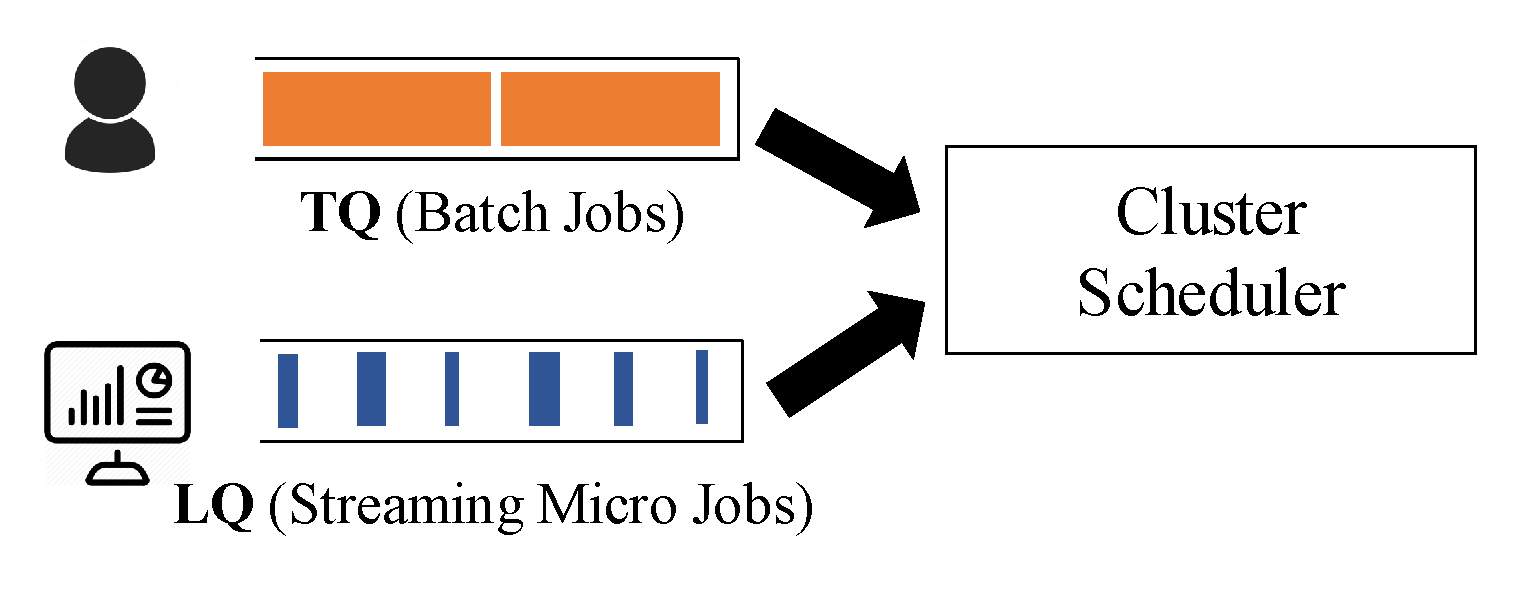
\includegraphics[width=0.8\columnwidth]{fig/queues.pdf}%
  \caption{\new{Users and automated processes submit throughput-sensitive (TQ) and latency-sensitive (LQ) to the same cluster.}}%
  \label{fig:queues}
 	\vspace{-0.1in}
\end{figure}

To address the diverse goals, today's schedulers are becoming more and more complex.
They are multi-resource \cite{drf, tetris, multiresource-mungchiang, orchestra, pacman}, DAG-aware \cite{aalo, tetris, spark}, and allow a variety of constraints \cite{late, quincy, mantri, choosy, delay-scheduling}. 
Given all these inputs, they optimize for objectives such as fairness \cite{drf, jaffe-maxmin, drfq, hdrf}, performance \cite{sjf}, efficiency \cite{tetris}, or different combinations of the three \cite{carbyne, graphene}.
However, all existing schedulers have one shortcoming in common: \emph{they force the same performance goal on all jobs while jobs may have distinct goals}, and therefore fail to provide performance guarantee in the presence of multiple types of workloads with different performance metrics. 
In fact, the performance of existing schedulers can be \emph{arbitrarily bad} for some workloads.

\begin{figure}[!t]
	\centering
	
\includegraphics[width=0.3\linewidth]{fig/b1_mov_legend} 
	\\
	\subfloat[DRF ensures instantaneous fairness, but increases the completion times of latency-sensitive jobs.]
  {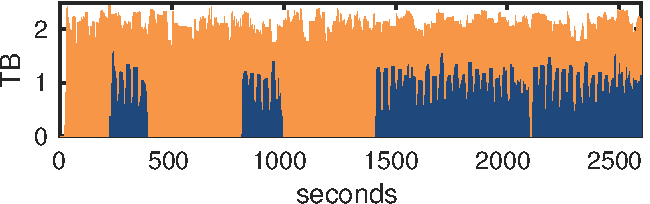
\includegraphics[width=0.85\linewidth]{fig/b1_mov_DRF_BB}\label{fig:motiv-DRF}}
	%\subfloat[DRF -- The completion time of 4 \burstq jobs are  202, 178, 715, and 719 seconds, respectively.]{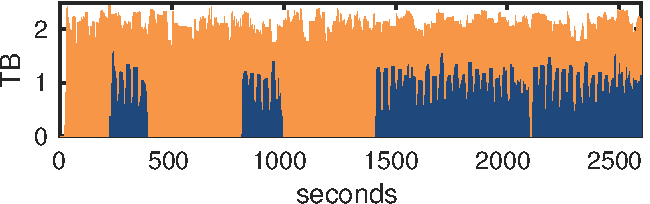
\includegraphics[width=1.0\linewidth]{fig/b1_mov_DRF_BB}\label{fig:motiv-DRF}}
	\\
	\subfloat[SP decreases completion times of latency-sensitive jobs, but throughput-sensitive batch jobs do not receive their fair shares.]
  {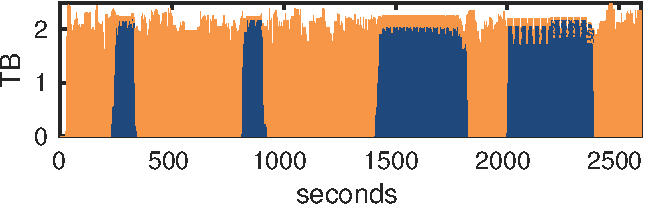
\includegraphics[width=0.85\linewidth]{fig/b1_mov_Strict_BB}\label{fig:motiv-Strict}}
	%\subfloat[Strict Prority (SP)-- The completion time of 4 \burstq jobs are  124, 121, 430, and 405 seconds, respectively.]{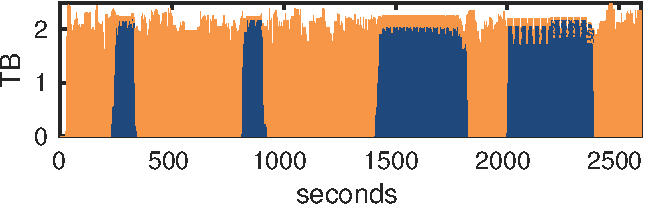
\includegraphics[width=1.0\linewidth]{fig/b1_mov_Strict_BB}\label{fig:motiv-Strict}	}
	\\
	\subfloat[The ideal solution allows first two latency-sensitive jobs to finish as quickly as possible, but protects batch jobs from latter \burstq jobs by ensuring long-term fairness.]
  {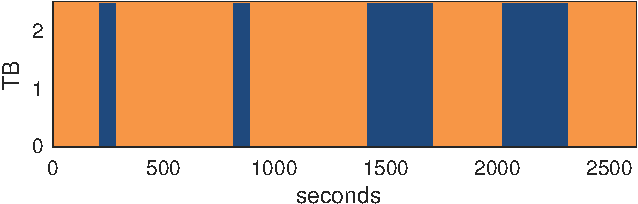
\includegraphics[width=0.85\linewidth]{fig/b1_mov_Optimum_BB}\label{fig:motiv-optimal}}	
	\caption{Need for bounded priority and long-term fairness in a shared multi-resource cluster with latency-sensitive (\burstq: blue/dark) and throughput-sensitive (\batchq: orange/light) jobs. \new{The blank part on the top is due to resource fragmentation and overheads in Apache YARN.}
    Although we focus only on memory allocations here, similar observations hold in multi-resource scenarios. \todo{put the memory (TB) instead of (TB) on the figures.}}
%    \todo{We should also have a figure showing the arrivals of LQ A.}
%    \mosharaf{Something is wrong with the third figure. Total area of blue should be the same regardless of algorithm.} 
%    \zhenhua{I didn't see the problem. The area for each arrival seems the same.}}
    %In DRF, it is unfair for the first two jobs to slow down their progress although they require very small resources. From 0 to 1400 seconds, Strict speeds up the delay-sensitive jobs from \burstq  but it later makes \batchq starving of resources because of the large jobs. \todo{change \burstq  and \batchq to \burstq  and \batchq}}
	\label{fig:motiv_ex}
		\vspace{-0.1in}
\end{figure}

Consider the simple example in Figure~\ref{fig:motiv_ex} that illustrates the inefficiencies of existing resource allocation policies, in particular, DRF~\cite{drf} and Strict Priority (SP) \cite{strict_priority} for coexisting workloads with different requirements. 
In this example, we run memory-bound jobs in 
\delete{Tez atop Apache YARN}
within a cluster of 40 nodes, where each node has 32 CPU cores and 64 GB RAM.
% 
There are two queues in the system, where each queue contains a number of jobs with the same performance goals.  
\new{Apache Hadoop YARN \cite{hadoop-fair-scheduler} is set up to manage the resource allocation among the queues.}
The first queue is for Spark streaming, which submits \delete{a number of MapReduce jobs }\new{a MapReduce job} every 10 minutes. 
We call it latency-sensitive queue (\burstq) because it aims to finish the jobs as quickly as possible.
The second queue is a throughout-sensitive batch-job queue (\batchq) formed by jobs generated from the BigBench workload~\cite{bbench} and queued up at the beginning. \batchq cares more about its long-term averaged resources received, e.g., every 10 minutes.
\todo{remove the TQ and LQ definition as they are defined in the Figure 1.}
For simplicity of exposition, all jobs are memory-bound. 
%While \burstq  tries to complete \emph{each job} as quickly as it arrives, \batchq cares more about its long-term averaged resources received, e.g., every 10 minutes.
% 
We consider two extreme classes of policies -- priority-based and fairness-based allocation -- in this example, where the former is optimized for latency and the latter for fairness.
% There are many other policies in between such as service curve and network calculus in general.
% Service curve and network calculus are often too conservative; \ie, they only admit a very small number of queues \cite{}.
Specifically, we focus on the inefficiency of DRF and SP. 
The memory resource consumption
%\footnote{The blank part on the top is due to resource fragmentation and overheads in Apache YARN.}
under these two policies is depicted in Figures~\ref{fig:motiv-DRF} and~\ref{fig:motiv-Strict}, respectively. 
We defer the discussion of other policies to Section~\ref{sec:property-analysis}. 
%\todo{We should add numbers about the completion time under two }
%\mosharaf{We should probably remove TQ and LQ names and just say latency- and throughput-sensitive jobs.}
%\zhenhua{Agreed. }

SP gives \burstq the whole cluster's resources (high priority) whenever it has jobs to run; hence, it provides the lowest possible response time. 
For the first two arrivals, the average response time is 130 seconds. 
A detrimental side effect of SP, however, is that there is no resource isolation -- \batchq jobs may not receive any resources at all! 
In particular, \burstq has incentives to increase its arrivals -- e.g., for more accurate sampling and more iterations in training neural networks -- without any punishment. 
As it does so from the third job arrival, \batchq no longer receives its fair share. 
In the worst case, \burstq can take all the system resources and \emph{starve} \batchq. 
In summary, SP provides the best response time for \burstq , but no isolation protection for \batchq at all.
In addition, SP is incapable of handling multiple {\burstq}s. 
% \zhenhua{Actually, when \burstq  increases its burst size, its response time goes worse!}

In contrast, DRF enforces \emph{instantaneous} fair allocation of resources at all times. 
During the burst of \burstq , \burstq  and \batchq share the bottleneck resource (memory) evenly until the jobs from \burstq  complete; then \batchq gets all resources before the next burst of \burstq . 
Clearly, \batchq is happy at the cost of longer completion times of \burstq 's jobs, whose response time increases by 1.6 times. 
In short, DRF provides the best isolation protection for \batchq, but no performance consideration for \burstq . 
When there are many {\batchq}s, the response time of \burstq  can be very large. 

%Therefore, it is natural to ask if we can achieve the best response time of {\burstq}s and fairness for {\batchq}s simultaneously. 
Clearly, it is impossible to achieve the best response time under \emph{instantaneous} fairness, which fully decides the allocation. 
In other words, there is a hard tradeoff between providing instantaneous fairness for {\batchq}s and minimizing the response time of {\burstq}s.
Consequently, we aim to answer the following fundamental question in this paper: \emph{how well can we simultaneously accommodate multiple classes of workloads with performance guarantees, in particular, isolation protection for {\batchq}s and low response times for {\burstq}s}? 

\begin{figure}[!t]
  \centering
  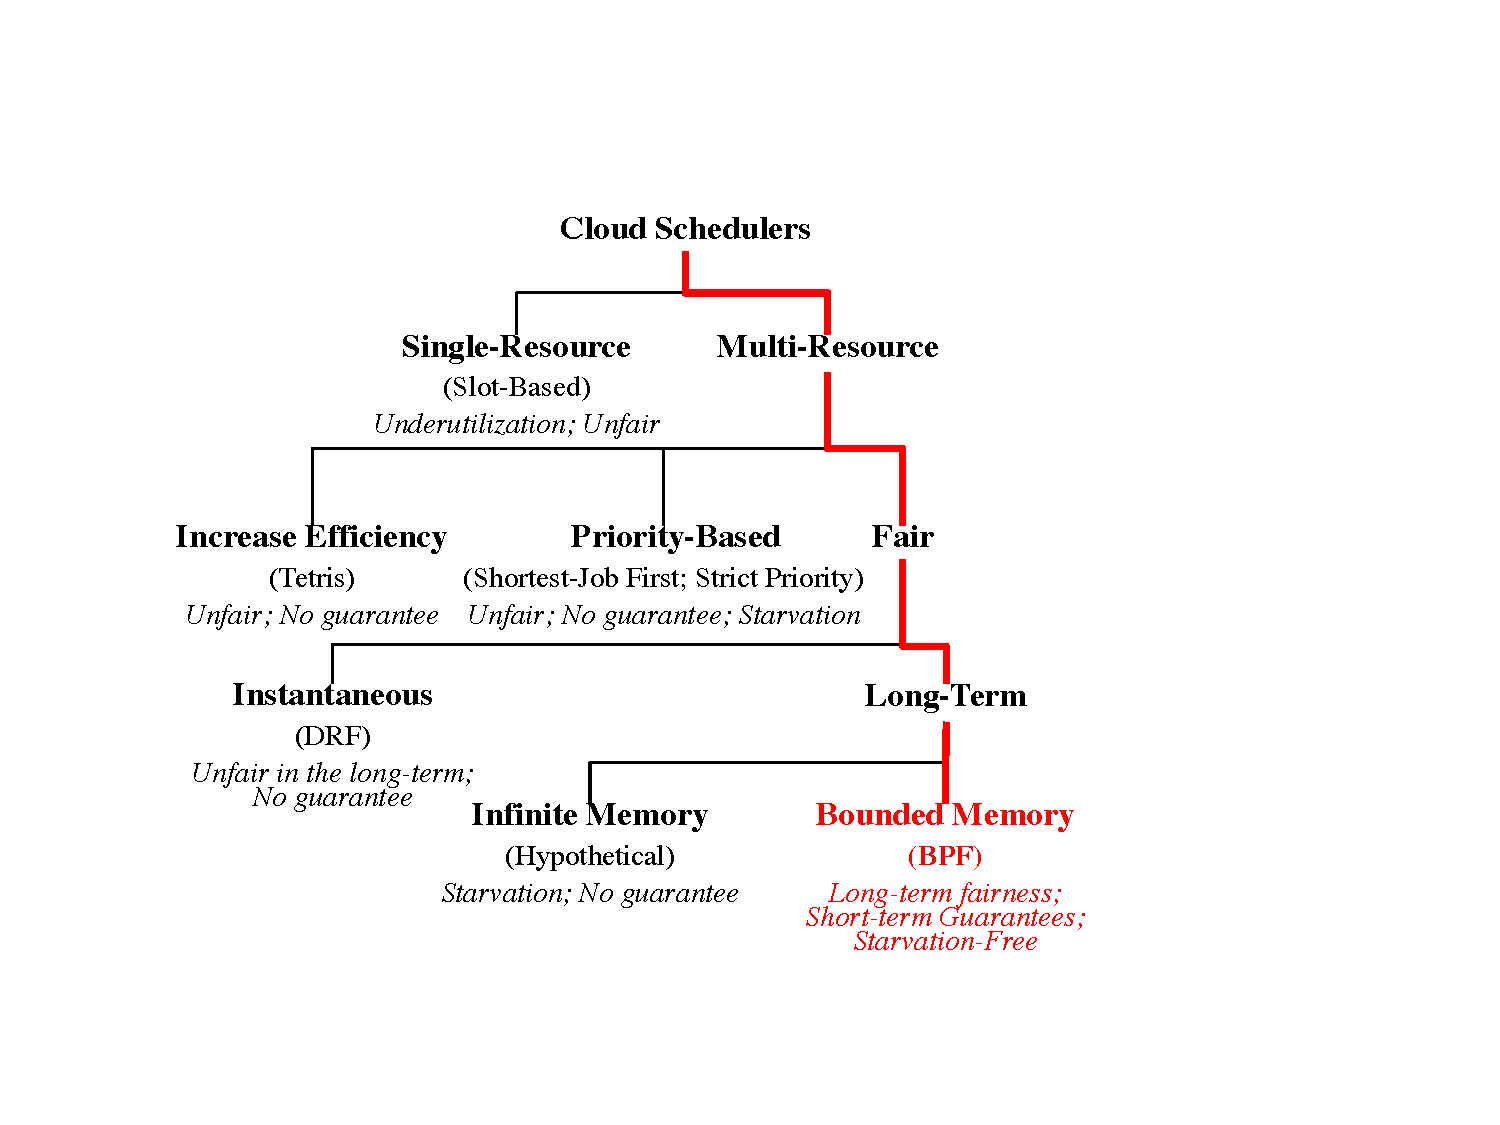
\includegraphics[width=0.85\linewidth]{fig/Design-Space.pdf}%
  \caption{{\name} in the cluster scheduling design space.}%
  \label{fig:design-space}
  	\vspace{-0.2in}
\end{figure}

We answer this question by designing \name: the first multi-resource scheduler that achieves both isolation protection for {\batchq}s in terms of \emph{long-term} fairness and response time guarantees for {\burstq}s, and is strategyproof. 
It is simple to implement and provides significant performance improvements even in the presence of uncertainties. 
The key idea is ``bounded'' priority for {\burstq}s: as long as the burst is not too large to hurt the long-term fair share of {\batchq}s, they are given higher priority so jobs can be completed as quickly as possible. 
Figure~\ref{fig:design-space} shows \name in the context of cluster scheduling landscape. 
%There are several challenges, and by solving them 
We make the following contributions.

\paragraph{Algorithm design.} We develop \name with the rigorously proven properties of strategyproofness, short-term bursts, long-term fairness, and high system utilization (\S\ref{sec:approach}). When {\burstq}s have different demands for each arrival, we further design mechanism to handle the uncertainties.

%\paragraph{Handling uncertainties.} We develop a simple yet efficient method to allow customers with significant estimation errors of their burst sizes to request the right amount of resources to satisfy their performance goals. We also highlight the difference between single-resource allocation and multi-resource allocation in the presence of estimation errors. In particular, we prove that the resource demands in the multi-resource scenario is always higher than those if resources are allocated individually unless there is no estimation error. This is true even when errors on different resources are independent. In addition, larger estimation errors lead to higher resource demands.
%\mosharaf{Didn't understand the last couple sentences, especially the phrase ``risk premium''.}
%\zhenhua{I adjusted. Let me know if it works.}

\paragraph{Design and implementation.} 
We have implemented \name on Apache YARN \cite{yarn} (\S\ref{sec:impl}).
Any framework that runs on YARN can take advantage of \name.
The \name scheduler is implemented as a new scheduler in Resource Manager that runs on the master node.
The scheduling overheads for admitting queues or allocating resources are negligibly less than 1 ms for 20,000 queues.


%
%We implement the system. One challenge is the delay in serving the bursts of {\burstq}s. \todo{Feel free to add more.}
%\mosharaf{This is probably not big enough to highlight here. Should be merged with the eval.}
%\zhenhua{That's fine. Just want to make sure it's mentioned.}

\paragraph{Evaluation based on both testbed experiments and large-scale simulations.}
In deployments, \name significantly provides up to $5.38\times$ lower completion times for \burstq jobs than DRF, while maintaining the same long-term fairness (\S\ref{sec:testbed}). 
At the same time, \name provides up to $3.05\times$ more fair allocation to {\batchq} jobs compared to SP.
%Furthermore, \name performs well even in the presence of demand variations and moderate misestimations (\S\ref{sec:sensitivity_analysis}).%\todo{sensitivity analysis regarding arrival time?}.
%\mosharaf{Not sure about talking about the preemption business here.}
%\zhenhua{Those are old texts. Feel free to edit.}

%
%\zhenhua{I'm not sure when to put the ideal allocation}
%\mosharaf{Following can be dropped.}
%The ideal allocation we target at is depicted in Figure~(\ref{fig:motiv-optimal}).
%Despite the negative result, the good news is that if we relax the instantaneous fairness to long-term fairness, both properties can be achieved at the same time. In fact, long-term fairness is good enough to provide the isolation protection to {\batchq}s. This is depicted in Figure~\ref{fig:motiv-optimal} as the ideal allocation. 
%The key idea is ``bounded'' priority for {\burstq}s: as long as the burst is not too large to hurt the fair share of {\batchq}s, they are given higher priority so jobs can be completed as quickly as possible. 
%In particular, before 1,400 seconds, \burstq 's bursts are small, so it gets higher priority, which is similar to SP. 
%After \burstq  increases its demand, only a fraction of its demand can be satisfied with the entire system's resources. Then it has to give resources back to \batchq to ensure the long-term fairness.
%
%
%=======old text=======
%
%
%Nowadays, there are multiple types of workloads with heterogeneous objectives. 
%(1) (Periodic) bursty workloads such as Spark streaming, scheduled tasks and routines. Their main goal is to minimize response time in seconds or even milliseconds.
%(2) Batch jobs. Long-term throughput measured in minutes or hours.
%(3) Interactive workloads. Non-periodic but can depend on response time, to minimize response time. Service curve is more suitable. 
%
%\thoughts{Is there a way to unify different objectives? Initial thoughts: demand can be represented by $d(t)$, where $t$ is discrete for presentation simplicity but can be easily extended to continuous case. Then $d(t)$ is nonzero at  periodic timeslots for (1), at one timeslot for (2), and at random timeslots for (3). Performance can be measured at each period for (1), after a sufficiently long interval for (2) as progress, and between consecutive arrivals for (3). Even though these workloads look different, there seems to be a way to unify them.}
%
%Under the cloud computing regime, either private or public, these workloads may share the same underlying physical infrastructure. 
%The resource contention among workloads leads to scheduling and resource allocation.
%In nowadays settings, there are multiple queues, each of which consists of a number of jobs. Each job can have multiple tasks potentially with interdependency.
%Jobs of the same queue belong to the same workload, and therefore have the same objective\footnote{A related concept is user. A user may have multiple queues, e.g., for different applications.}.
%Each queue has a weight and needs isolation guarantee. 
%Jobs may be large, e.g., for throughput-sensitive workloads. In this case, their progress can be measured by the number of tasks served within a time interval. \zhenhua{We need to clarify this to be consistent with the numerics.}
%\mosharaf{Is it possible to talk about things without introducing queues first? Then introducing queues. Btw, we should look up the Jockey paper from EuroSys 2012 carefully.}
%
%Despite the heterogeneity, start-of-the-art schedulers force the same performance goal on all workloads, which incurs inefficiency.
%
%Consider the example of a system serving both throughput-sensitive and latency-sensitive workloads. In this example, the number of tasks completed within a time interval is used to capture the progress of a throughout-sensitive batch-job queue (\batchq) \cite{tetris, carbyne, mantri, late}.
%Interactive sessions and streaming applications form latency-sensitive queues (\burstq): each \burstq is a sequence of small jobs following an ON-OFF pattern. \zhenhua{It's not really a ON-OFF pattern. It's more like a periodic arrival with deadlines...}
%For these jobs \cite{spark-streaming, spark, splunk-analysis, presto}, individual completion times or latencies are far more important than the throughput of the \burstq. 
%\mosharaf{I agree. We should get rid of this ON-OFF part. Another thing to do would be getting rid of asking for period lengths from users.}
%
%\todo{add an example to show the problem.}
%
%There are two classes of schedulers in literature, but neither of them solved the problem completely.
%\mosharaf{There is a third category that focuses on increasing utilization.}
%
%Priority-based: good for \burstq, while \batchq can be starved
%
%Fairness-based such as DRF: good for \batchq, while response time of \burstq can be arbitrarily worse compared to the optimal solution (one \burstq, $n$ {\batchq}s, $n$ goes to infinity)
%
%Other solutions: BVT, Carbyne \zhenhua{Any others? We need to discuss all of them, perhaps in the motivation section}
%\mosharaf{We may need to update the taxonomy as well.}
%
%Therefore, we ponder a fundamental question: \emph{can we enable latency-sensitive {\burstq}s and throughput-sensitive {\batchq}s to coexist, where {\burstq}s are permitted short-term resource bursts while ensuring long-term fairness between the two, as well as maximizing {\burstq}s served with resource guarantees?}
%
%In this paper, we first show that there is a hard tradeoff between instantaneous fairness and short-term resource bursts. 
%
%Then we relax the fairness notion from instantaneous one to long-term one and the key opportunity emerges: {\batchq}s do not care about allocated resources in the short term, as long as the long-term averaged resource share remains the same. This temporal flexibility allows us to accommodate bursts of {\burstq}s without hurting {\batchq}s. 
%
%However, naive admission control may result in very few {\burstq}s admitted with resource guarantees, leading to suboptimal performance for {\burstq}s even with a high system utilization.
%
%In addition, there are challenges for multi-resource allocation \zhenhua{is this trivial?} and handling the uncertainties.
%
%%\textcolor{blue}{
%%Additionally, how one reasons about system utilization becomes more complicated in the presence of both {\burstq}s and {\batchq}s. 
%%While it is relatively easy to fill the cluster with many batch jobs to achieve high utilization, {\burstq}s often have higher value and are harder to accommodate with resource guarantees. 
%%Compared to a simple solution that rejects most of {\burstq}s and/or serves them with best efforts, system operators are likely to prefer to maximize the {\burstq}s served with resource guarantees, which leads to more predictable performance. %We call the resources allocated to {\burstq}s with resource guarantees {\burstq} utilization.
%%%}
%%}
%%
%%
%%The challenges are \zhenhua{we should add some key messages from theoretical results. My current thoughts are: BG and LF seem not very challenging given the opportunity we discussed in the last paragraph, so we should focus on strategyproofness and (LQ) utilization. Xiao, as you have some concerns regarding the strategyproofness, can you write down your thoughts here? If BPF in the current form is strategyproof, then we should highlight some other alternatives are not, similar to our HUG paper. Otherwise, we should improve BPF and use the current version as the example. I can write something along our NSF proposal regarding the tradeoff between progress and utilization. I looked into our HUG paper, and it seems the intro has quite a few strong points, such as DRF's utilization can be arbitrarily low, naive work conservation can lead to worse utilization, etc. Meanwhile, the elastic demand is very clear. We should try to do something similar. }
%%
%%
%%
%%\textcolor{blue}{
%%The need to separate throughput- and latency-sensitive job queues in big data clusters is akin to the classic networking problem of supporting throughput-sensitive flows and latency-sensitive realtime communication on network access links \cite{cbq, intserv-hierarchy, hfsc, cruz-sc}.
%%The key difference between the two is the multi-resource nature of cluster scheduling and challenges arising from it. 
%%We aim for a solution that can be applied to multi-resource clusters.
%%}
%
%\textcolor{blue}{
%%\todo{five properties, but some are missing below.}
%In this paper, we first explore opportunities and challenges in achieving four desired properties in this context (\S\ref{sec:motivation}): (i) allowing {\burstq}s to enjoy short-term high resource usage during their ON periods to minimize \emph{individual} job response times; (ii) maintaining the same \emph{long-term} fairness as existing multi-resource fair allocation policies by preventing arbitrarily large bursts; (iii) maximizing system utilization and {\burstq}s served with resource guarantees; %\new{(iv) It is better off sharing than using static sharing}. 
%and (iv) the policy needs to be strategyproof because otherwise {\burstq}s may lie about their demands to gain more resources. 
%}
%
%\subsection*{Contributions}
%
%\paragraph{Algorithm development.} properties with rigorous proofs: strategyproofness, short-term bursts, long-term fairness, system utilization
%
%\paragraph{Design and implementation.} any challenges here? The slow start problem that Tan is currently working on is one potential.
%
%\paragraph{Evaluation based on both testbed experiments and large-scale simulations.}
%In deployments, \name significantly provides up to $5.38\times$ (totally 9 queues in a cluster) faster performance with smaller variation for \burstq jobs than DRF, while maintaining the fairness among the queues (\S\ref{sec:testbed}). 
%\name protects the {\batchq} jobs up to $3.05\times$ compared to SP.
%Furthermore, \name performs well even in the presence of moderate misestimations of task demands and without preemption allowed (\S\ref{sec:sensitivity_analysis})\todo{sensitivity analysis regarding arrival time?}.
%
%\section{Motivation}
%
%\mosharaf{If we could talk about some numbers that'd be good. Of course, we don't have any real traces ourselves. One possible option is going through existing works and see if they mention any high-level characteristics that we can use.}
%\zhenhua{I agree. While searching for existing work, we can start from some simple examples as we did in the HUG paper, which is well received.}
%
%\subsection{Problem Formulation}
%
%\subsection{Desired Properties}
%
%\subsection{Challenges and Inefficiencies of Existing
%Allocation Policies}
%
%SP
%
%DRF
%
%BVT
%
%Carbyne
%
%others?
%
%\subsection{Hard tradeoff between instantaneous fairness and bursty accommodations}
%
%\subsection{Naive admission control results in few {\burstq}s admitted with performance guarantee}
%
%\subsection{Estimation errors matter}
%
%
%\section{\name: analytical results}
%
%The \name algorithm
%
%long-term fairness
%
%burst guarantee
%
%Pareto efficiency
%
%strategyproofness
%
%\section{Stochastic optimization to handle the uncertainties}
%\zhenhua{Xiao is working on this}
%
%Model
%
%Algorithm
%
%
%\section{System design}
%
%Reducing overheads from creating containers. \zhenhua{Tan is looking into this}
%
%\section{Evaluations}
%
%\zhenhua{Tan, can you add the current figure list here?}
%
%\todo{Everyone, please add to the figure list addition figures that may help.}
%
%
%We discuss related work in Section~\ref{sec:related}.

%\mosharaf{A list of three contributions? Problem formulation, Algorithm and its properties, and full system evaluation and thorough eval.}
